\section{Rainfall}
Written by Amato Van Geyt

The goal of this was identifying different anomalies in the rainfall in the USA in a given time period. The time period we choose was 1970 until 2013 as the used datasets seemed to have the most available and reliable data in this period. \\ 

\subsection{The Used Datasets}
The used dataset was initially the original noaa-dataset (\url{ftp://ftp.ncdc.noaa.gov/pub/data/noaa/}) but many problems were encountered with this dataset, especially for the rainfall. First of all was all the data organised by year which made it hard to debug as for finding anomalies we need to be able to quickly compare a certain value with values at the same place but at different times, something this dataset hindered us in. The records themselves were also very chaotically organised and contained much useless information giving cause to long and error-prone processing. The worst of all though was the fact that the rainfall wasn't given per day but for a certain time-period expressed in hours. As this time-period varied a lot among the different weather-stations or even for the same time-period and as there were gaps of data this gave cause to very erratic results. This gave cause to choosing for a new dataset which was aggregated on the previous one. \\ 
The new dataset (\url{ftp://ftp.ncdc.noaa.gov/pub/data/ghcn/daily/}) contained essentially the same data but sorted by weather-station (one file per station) and each line of that file told us exactly the daily values for a certain weather measure for a given month of a given year. This allowed for very easy parsing and processing. The files were much smaller as well and easier for debugging. The final results are based on this data and can be seen on the site.\\ 

\subsection{Obtaining the results}
The way how the results are obtained is simple. By using two phases of MapReduce we identify for every station the average and standard deviation of all the values over all the years in the data. This can be done for the value per day, or the value per month, which is the average of all daily values. As there was still some 'dirty' or missing data we did some filtering on the quality before using it in our computation. And if saw that the amount of data used to calculate the standard deviation and average was too small, we dropped it as it was too error-prone. Then we used a parameter, entered via the command line to determine what we would see as an anomaly and what not. This value would be the amount of standard deviations the value had to be away from the average to be seen as an anomaly. After some experimenting we saw that the best value for our daily anomalies was 6 and for our monthly anomalies 3. Our final output was a text file per weather station which contained all the anomalies we found for it, one per record. The record contained the time, the station-ID, the value, the standard deviation and its normal average value. \\

\subsection{Postprocessing the results for visualisation}
As this did not contain the coordinates of the station and the name of the station yet we had to make an additional MapReduce-phase which took our previous output as input and added this additional data to every record while also re-organising it. The last step we had to do after this was to do another processing step in order to visualize it on a map. In order to do this, in an uniform way with the other parts of the project, we use GeoJSON. After this was done, the only thing remained was plugging it into the already existing map, doing some small modifications with a Python-script. The final result can be seen in Figure \ref{fig:rainfall1}. The anomaly found in it was indeed an anomaly as the hurricane Emily made a passage through North Carolina during those days, as shown in the Wikipedia-report in Figure \ref{fig:rainfall2}.
\begin{figure}[ht]
\centering
\makebox[\textwidth][c]{
  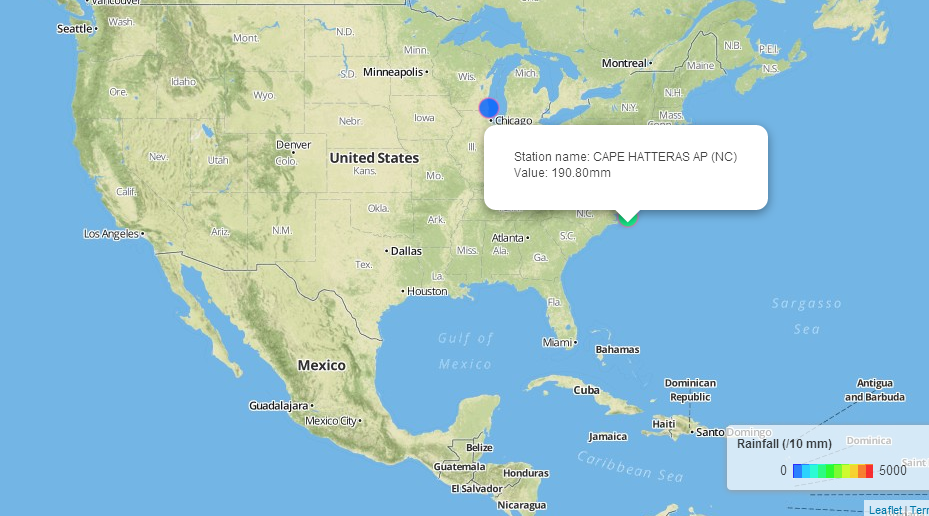
\includegraphics[width=17cm]{figures/rainfall1.png}
}
\caption{The rainfall anomalies on 31/08/1993}
\label{fig:rainfall1}
\end{figure}
\begin{figure}[ht]
\centering
\makebox[\textwidth][c]{
  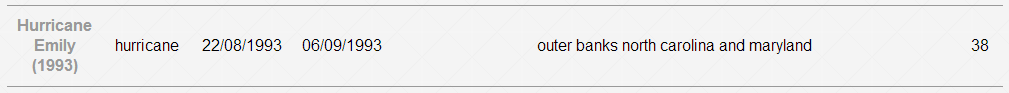
\includegraphics[width=17cm]{figures/rainfall2.png}
}
\caption{The wikipedia-report of hurricane Emily}
\label{fig:rainfall2}
\end{figure}
